\documentclass{standalone}
\usepackage{pgfplots}
\pgfplotsset{width=7cm,compat=1.8}

\begin{document}
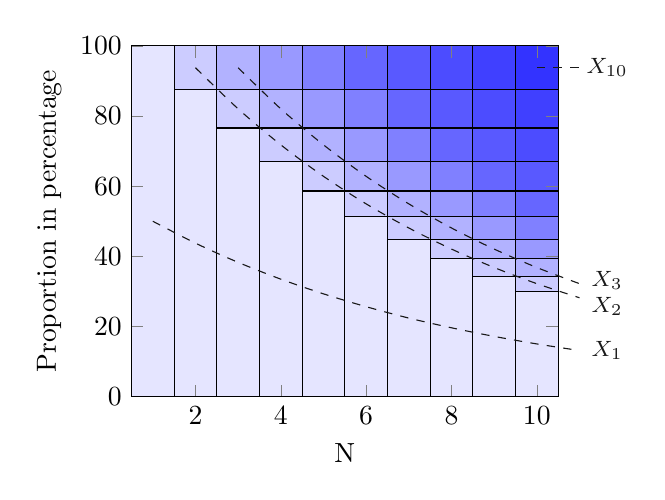
\begin{tikzpicture}
\begin{axis}[
  ybar stacked,
  bar width=1,
  axis on top,
  xmin=0.5,
  xmax=10.5,
  ymin=0,
  ymax=100,
  xlabel={N},
  ylabel={Proportion in percentage},
  after end axis/.code={
    \draw [color=black!90!white,dashed,smooth] plot coordinates{(axis cs:1,50) (axis cs:2,43.75) (axis cs:3,38.28125) (axis cs:4,33.496) (axis cs:5,29.309) (axis cs:6,25.646) (axis cs:7,22.4) (axis cs:8,19.635) (axis cs:9,17.181) (axis cs:10,15.033) (axis cs:11,13.154)} node [xshift=1em,font=\footnotesize] {$X_1$};
    \draw [color=black!90!white,dashed,smooth] plot coordinates{(axis cs:2,93.75) (axis cs:3,82.031) (axis cs:4,71.777) (axis cs:5,62.805) (axis cs:6,54.954) (axis cs:7,48.086) (axis cs:8,42.075) (axis cs:9,36.816) (axis cs:10,32.213) (axis cs:11,28.187)} node [xshift=1em,yshift=-0.75ex,font=\footnotesize] {$X_2$};
    \draw [color=black!90!white,dashed,smooth] plot coordinates{(axis cs:3,93.75) (axis cs:4,82.031) (axis cs:5,71.777) (axis cs:6,62.805) (axis cs:7,54.954) (axis cs:8,48.086) (axis cs:9,42.075) (axis cs:10,36.816) (axis cs:11,32.213)} node [xshift=1em,yshift=0.25ex,font=\footnotesize] {$X_3$};
    \draw [color=black!90!white,dashed,smooth] plot coordinates{(axis cs:10,93.75) (axis cs:11,93.75)} node [xshift=1em,font=\footnotesize] {$X_{10}$};
  }
  ]
\addplot[fill=blue!10!white] coordinates {(1,100) (2,87.500) (3,76.562) (4,66.992) (5,58.618) (6,51.291) (7,44.880) (8,39.270) (9,34.361) (10,30.066)};
\addplot[fill=blue!20!white] coordinates {(1,0) (2,12.500) (3,10.938) (4,09.570) (5,08.374) (6,07.327) (7,06.411) (8,05.610) (9,04.909) (10,04.295)};
\addplot[fill=blue!30!white] coordinates {(1,0) (2,0.00000) (3,12.500) (4,10.938) (5,09.570) (6,08.374) (7,07.327) (8,06.411) (9,05.610) (10,04.909)};
\addplot[fill=blue!40!white] coordinates {(1,0) (2,0.00000) (3,0.00000) (4,12.500) (5,10.938) (6,09.570) (7,08.374) (8,07.327) (9,06.411) (10,05.610)};
\addplot[fill=blue!50!white] coordinates {(1,0) (2,0.00000) (3,0.00000) (4,0.00000) (5,12.500) (6,10.938) (7,09.570) (8,08.374) (9,07.327) (10,06.411)};
\addplot[fill=blue!60!white] coordinates {(1,0) (2,0.00000) (3,0.00000) (4,0.00000) (5,0.00000) (6,12.500) (7,10.938) (8,09.570) (9,08.374) (10,07.327)};
\addplot[fill=blue!65!white] coordinates {(1,0) (2,0.00000) (3,0.00000) (4,0.00000) (5,0.00000) (6,0.00000) (7,12.500) (8,10.938) (9,09.570) (10,08.374)};
\addplot[fill=blue!70!white] coordinates {(1,0) (2,0.00000) (3,0.00000) (4,0.00000) (5,0.00000) (6,0.00000) (7,0.00000) (8,12.500) (9,10.938) (10,09.570)};
\addplot[fill=blue!75!white] coordinates {(1,0) (2,0.00000) (3,0.00000) (4,0.00000) (5,0.00000) (6,0.00000) (7,0.00000) (8,0.00000) (9,12.500) (10,10.938)};
\addplot[fill=blue!80!white] coordinates {(1,0) (2,0.00000) (3,0.00000) (4,0.00000) (5,0.00000) (6,0.00000) (7,0.00000) (8,0.00000) (9,0.00000) (10,12.500)};
\addplot[fill=blue!85!white] coordinates {(1,0) (2,0.00000) (3,0.00000) (4,0.00000) (5,0.00000) (6,0.00000) (7,0.00000) (8,0.00000) (9,0.00000) (10,0.00000)};
\end{axis}
\end{tikzpicture}
\end{document}
